\documentclass{beamer}

\mode<presentation>
{
  \usetheme{Madrid}      % or try Darmstadt, Madrid, Warsaw, ...
  \setbeamertemplate{navigation symbols}{}
  \setbeamertemplate{caption}[numbered]
} 

\colorlet{beamer@blendedblue}{black}

\usepackage[french]{babel}
\usepackage[utf8]{inputenc}
\usepackage[T1]{fontenc}
%\usepackage[squaren,cdot]{SIunits}
\usepackage{graphicx}
\usepackage{listings}

\graphicspath{}

\logo{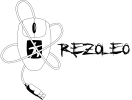
\includegraphics[height=0.8cm]{rezoleo.png}\vspace{10pt}\hspace{20pt}}
\title{Couche liaison}
\author{LEDER "Ziman" Simon}
\institute{Rezoleo\\}
\date{\today}

\begin{document}
	
	\begin{frame}
		\titlepage
	\end{frame}
	
	\begin{frame}
		\frametitle{Sommaire}
			\tableofcontents
	\end{frame}
	
\section{Introduction}

	\begin{frame}{Introduction}{Sous-couche}
		Elle de divise en deux sous-liaison : MAC et LLC \\
		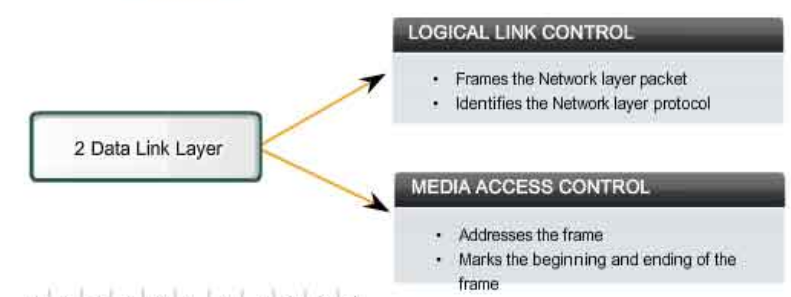
\includegraphics[scale=0.4]{macllc.png}
	\end{frame}

	\begin{frame}{Introduction}{Rôle}
		Les bits à envoyer sont regroupés en trames binaires.\\

		\begin{itemize}
			\item [\textbullet] \textbf{La sous-couche MAC} : Elle gère l'accès au support de transmission, commun à toutes les machines connectées.
			\item [\textbullet] \textbf{La sous-couche LLC} : Elle gère la gestion du trafic, le contrôle d'erreur \\
		\end{itemize}

		La couche de liaison de données s'occupe de la livraison locale de trames entre dispositifs présents sur un même LAN.

	\end{frame}

\section{Adressage MAC}

	\begin{frame}{Adressage MAC}{Rôle}

		\begin{itemize}
			\item [\textbullet] Reconnaître le début et la fin des trames dans le flux binaire reçu de la couche physique ;
			\item [\textbullet] Délimiter les trames envoyées en insérant des informations (comme des bits supplémentaires) dans ou entre celles-ci, afin que leur destinataire puisse en déterminer le début et la fin ;
			\item [\textbullet] Détecter les erreurs de transmission, par exemple à l'aide d'une somme de contrôle (checksum) insérée par l'émetteur et vérifiée par le récepteur ;
			\item [\textbullet] Insérer les adresses MAC de source et de destination dans chaque trame transmise ;
			\item [\textbullet] Filtrer les trames reçues en ne gardant que celles qui lui sont destinées, en vérifiant leur adresse MAC de destination ; 
			\item [\textbullet] Contrôler l'accès au média physique lorsque celui-ci est partagé.
		\end{itemize}
	\end{frame}

	\begin{frame}{Adressage MAC}{L'adresse}
		Une adresse MAC est une suite de 6 octets (48 bits) souvent représentée sous la forme hexadécimale 5E:FF:56:A2:AF:15. qui identifie de façon unique chaque interface réseau. \\
	\end{frame}

		\begin{frame}{Adressage MAC}{Adresses particulières}		

			\begin{table}[]
				\centering
				\begin{tabular}{|l|l|lll}
					\cline{1-2}
					FF:FF:FF:FF:FF:FF & Adresse broadcast                                                     &  &  &  \\ \cline{1-2}
					01:00:0C:CC:CC:CC & \begin{tabular}[c]{@{}l@{}}Cisco\\ 			Discovery Protocol\end{tabular} &  &  &  \\ \cline{1-2}
					01:80:C2:00:00:00 & \begin{tabular}[c]{@{}l@{}}Spanning\\ 			Tree Protocol\end{tabular}   &  &  &  \\ \cline{1-2}
					33:33:xx:xx:xx:xx & \begin{tabular}[c]{@{}l@{}}Adresses\\ 			multicast IPv6\end{tabular}  &  &  &  \\ \cline{1-2}
					01:5E:00:xx:xx:xx & \begin{tabular}[c]{@{}l@{}}Adresses\\ 			multicast IPv4\end{tabular}  &  &  &  \\ \cline{1-2}
					00:00:0c:07:ac:xx & Adresses HSRP                                                         &  &  &  \\ \cline{1-2}
					00:00:5E:00:01:XX & Adresses VRRP                                                         &  &  &  \\ \cline{1-2}
					\end{tabular}
				\end{table}
	\end{frame}


\section{Trame ethernet}

	\begin{frame}{Protocole Ethernet}{Trame ethernet}
		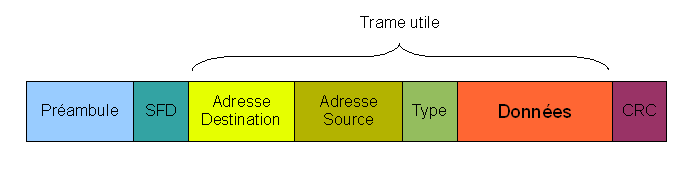
\includegraphics[scale=0.7]{trame.png}
	\end{frame}

	\begin{frame}{Protocole Ethernet}{Trame ethernet}
		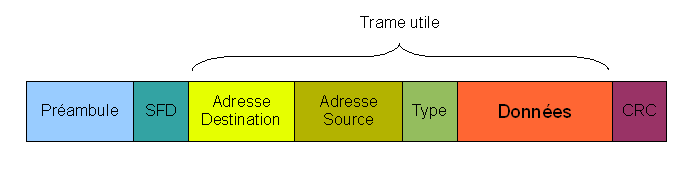
\includegraphics[scale=0.7]{trame.png}
		\textbf{Préambule :} Sept octets valant 10101010 (ou AA) sont utilisés dans ce but, ce qui fournit pendant 5,6 $\mu$s une onde rectangulaire de 5 MHz permettant d'acquérir la synchronisation bit.
	\end{frame}

	\begin{frame}{Protocole Ethernet}{Trame ethernet}
		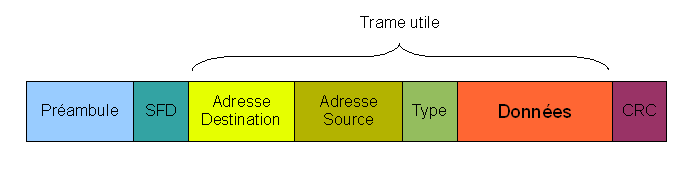
\includegraphics[scale=0.7]{trame.png}
		\textbf{SFD :} Une fois synchronisé, l'émetteur doit reconnaître le Délimiteur de trame qui lui indique le début des données utiles. Il vaut 10101011. (ou AB)
	\end{frame}

	\begin{frame}{Protocole Ethernet}{Trame ethernet}
		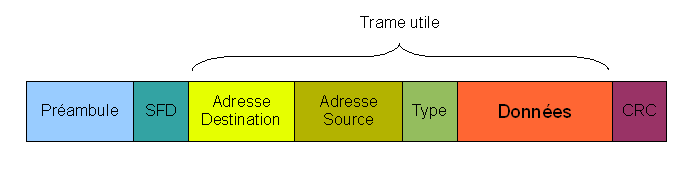
\includegraphics[scale=0.7]{trame.png}
		\textbf{Adresse MAC de Destination} \\
		\textbf{Adresse MAC Source}
	\end{frame}

	\begin{frame}{Protocole Ethernet}{Trame ethernet}
		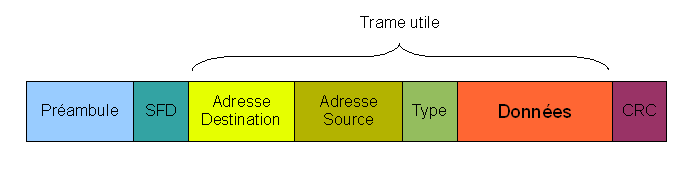
\includegraphics[scale=0.7]{trame.png}
		\textbf{Types de trames Ethernet et champ EtherType :} Type de protocole ou Longueur DATA 
	\end{frame}

	\begin{frame}{Protocole Ethernet}{Trame ethernet}
		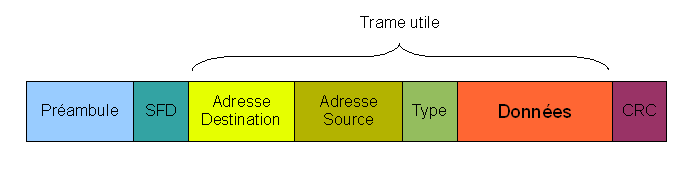
\includegraphics[scale=0.7]{trame.png}
		\textbf{Types de trames Ethernet et champ EtherType :} Type de protocole ou Longueur DATA 
	\end{frame}

	\begin{frame}{Protocole Ethernet}{Trame ethernet}
		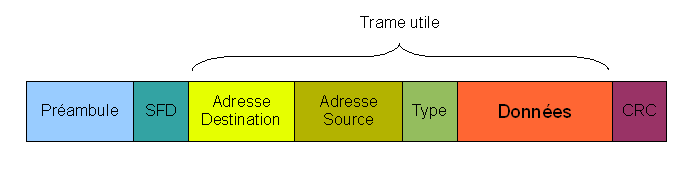
\includegraphics[scale=0.7]{trame.png}
		\textbf{Le contrôle d’erreur ou FCS pour Frame Control Sequence  :} Type de protocole ou Longueur DATA 
	\end{frame}

\section{Autres protocoles}

	\begin{frame}{Autres protocole}
		\begin{itemize}
			\item [\textbullet] Wi-fi
			\item [\textbullet] ATM
			\item [\textbullet] ZigBee
			\item [\textbullet] Bluetooth
		\end{itemize} 
	\end{frame}



\end{document}
